\documentclass{beamer}
%\documentclass[handout]{beamer}

%\usetheme{Pittsburgh}
\beamertemplatenavigationsymbolsempty
%\setbeamertemplate{footline}[frame number]
%\setbeamertemplate{footline}{\hspace*{.5cm}\tiny{\insertshorttitle \hspace*{50pt} \hfill\insertframenumber/\inserttotalframenumber\hspace*{.5cm}} \vspace{2pt}}
\setbeamertemplate{footline}{\hspace*{.5cm}\tiny{\, \hspace*{50pt} \hfill\insertframenumber/\inserttotalframenumber\hspace*{.5cm}} \vspace{2pt}}

\mode<handout>{
\usepackage{pgfpages}
\pgfpagesuselayout{2 on 1}[a4paper,border shrink=4mm]
%% \pgfpagesuselayout{4 on 1}[a4paper,landscape,border shrink=2mm]
}

\usepackage{subfigure}
\usepackage{float}
\usepackage{movie15}
\usepackage{color}
\usepackage{tabularx}
\usepackage{multirow}
\usepackage{multicol}
%\newcommand{\myurl}[1]{\href{http://#1}{#1}}
\usepackage{url}
\usepackage{hyperref}
\hypersetup{colorlinks=true,linkcolor=red,citecolor=green,filecolor=magenta,urlcolor=blue}

\definecolor{blue}{rgb}{0.0,0.0,0.55}
\definecolor{darkblue}{rgb}{0.10,0.10,0.70}

\definecolor{red}{rgb}{1.0,0.0,0.0}
\definecolor{darkred}{rgb}{0.75,0.0,0.0}

\definecolor{green}{rgb}{0.0,0.80,0.0}
\definecolor{darkgreen}{rgb}{0.0,0.5,0.0}

\definecolor{dimmed}{rgb}{0.8,0.8,0.8}
\mode<beamer>{
\setbeamercolor{math text}{fg=darkblue}
\setbeamercolor{local structure}{fg=black}
}

\mode<handout>{
\setbeamercolor{math text}{fg=black}
%% \setbeamercolor{structure}{fg=black}
\setbeamercolor{local structure}{fg=black}
}

% graphics (png, pdf, ...) NOT eps (to convert to pdf with epstopdf)
\usepackage{graphicx}

% list of path for graphics (Warning: the / at the end of each path is important)
\graphicspath{{graphics/}{graphics/logo/}{graphics/fingervein/}{graphics/biometrics/}{graphics/biometric-group/}}

\DeclareGraphicsExtensions{.pdf,.jpg,.png}



% default, triangle, circle, square et ball
%\setbeamertemplate{itemize item}[triangle]
\setbeamertemplate{itemize item}[circle]
\setbeamertemplate{itemize subitem}[circle]
\setbeamertemplate{enumerate item}[square]
\setbeamertemplate{enumerate subitem}[circle]

\begin{document}
% TITLE
\title[AMI and Bob]{AMI database and Introduction to Bob} 
%\subtitle{Biometric recognition} 
% AUTHOR
\author[A. Komaty -- Idiap 2016]{\textbf{Alain Komaty}\\ 
PostDoc at the Biometrics groups
} 


% INSTITUTE
\institute{

\includegraphics[scale=0.3]{idiap}


\includegraphics[scale=0.6]{Biometrics-logo}
} 

% DATE
\date{\today} 
% TITLE PAGE
\frame{\titlepage} % fancy title page

%\frame{\frametitle{Outline}\tableofcontents}
\begin{frame}

  \frametitle{AMI database}
  The AMI Meeting Corpus consists of:
  \begin{center}
    \begin{itemize}
      \item 100 hours of meeting recordings
      \item Include close-talking and far-field microphones
      \item Individual and room-view video cameras
      \item Output from a slide projector and an electronic whiteboard
    \end{itemize}
  \end{center}
The meetings were recorded in English using three different rooms with different acoustic properties, and include mostly non-native speakers$^1$.
\footnotetext[1]{\textit{http://groups.inf.ed.ac.uk/ami/corpus/overview.shtml}}
\end{frame}

\begin{frame}

  \frametitle{AMI database}
  The AMI Meeting Corpus Annotations:
  \begin{center}
    \begin{itemize}
      \item Linguistic
        \begin{itemize}
          \item high quality, manually produced orthographic transcription for each individual speaker
          \item word-level timings
        \end{itemize}
      \item behaviours
        \begin{itemize}
          \item dialogue acts
          \item word-level timings, topic segmentation
          \item extractive and abstractive summaries
          \item the types of head gesture, hand gesture, and gaze direction
        \end{itemize}      

    \end{itemize}
  \end{center}
The meetings were recorded in English using three different rooms with different acoustic properties, and include mostly non-native speakers$^1$.

\end{frame}

%
% SECTION
%\section{Biometric group}

%%
%% At least 2 slides but plan extra slides for discussion
%%

%% 1 slide on you
\frame{\frametitle{CV}
\begin{block}{Education}
% 2 items max
\begin{itemize}
\item PhD in Signal Processing, French naval Academy Research Institute - France - 2014
\item MSc in Signal Processing, UBO-ENSTA-Telecom Bretagne - France - 2010
\item BE from the Lebanese University, 2010
\end{itemize}
\end{block}

\begin{block}{Research topics}
\begin{itemize}
\item Signal processing, filtering, underwater acoustics, source localisation ...
\item Recently: Machine learning and speaker diarization.
\end{itemize}
\end{block}

%\begin{block}{Scientific contributions}
%\begin{itemize}
%\item h-index (3) \url{https://scholar.google.ch/citations?user=aeIX3V0AAAAJ&hl=fr}
%\item 12 (journals and conference papers)
%\end{itemize}
%\end{block}
}

% 1 slide on 1 research topic
\frame{\frametitle{Research topic}
\begin{block}{Enhanced Online Speaker Diarization}
\begin{itemize}
\item Integrate the inherent temporal structure of interactions between speakers.
\item Adapt state-of-the-art techniques to speaker diarization (such as i-vectors and deep learning).
\item Explore supervised and unsupervised domain adaptation techniques.
\end{itemize}
\end{block}

%\begin{block}{Research question(s)}
%\begin{itemize}
%\item Is there any of the abovementioned ambitious objectives not feasable?
%\end{itemize}
%\end{block}

%\begin{block}{Findings / Results}
%No results yet.
%\end{block}
}

%\frame{\frametitle{Research topic}
%\vspace{-1.5cm}
%\begin{figure}[htbp]
%\begin{center}
%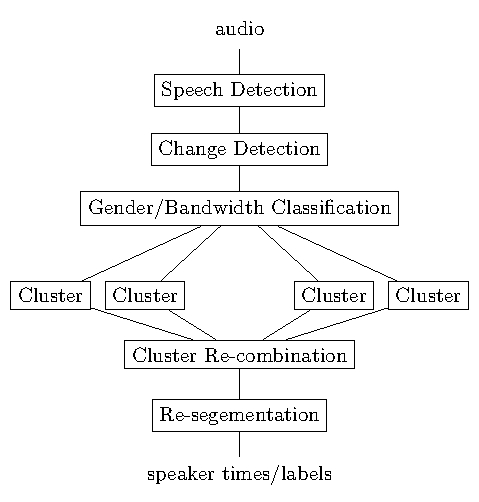
\includegraphics[width=0.65\textwidth]{Diagram_Speaker_diarization}
%\end{center}
%\caption{Prototypical speaker diarization system [Trantfer, 2006]}
%\label{Fig:Speaker_Rec}
%\end{figure}
%\vspace{-0.2cm}
%\scalebox{.4}{S. E. Tranter and D. A. Reynolds, "An overview of automatic speaker diarization systems," in IEEE Trans. on ASLP, vol. 14, no. 5, pp. 1557-1565, Sept. 2006.}

%}


% Additional slides for discussion
%\frame{\frametitle{Research topic}
%\begin{block}{...}
%\end{block}
%}




\begin{frame}

  \frametitle{Reproducible Research: A Motivation}

  \begin{center}
    \pgfimage[width=0.48\textwidth]{graphics/equations}%
    \hspace{1em}%
    \pgfimage[width=0.48\textwidth]{graphics/plots}%
    \vspace{1em}
  \end{center}

\end{frame}


\begin{frame}

  \frametitle{You Ask the Author for Clues...}

  You get:

  \only<2->{
    \vspace{1em}

    \begin{center}
      
\includegraphics[height=0.6\textheight]{graphics/short-question-mark}
    \end{center}
  }

\end{frame}


\begin{frame}
  \frametitle{Let's interact...}

  \only<1>{
    \begin{center}
    \pgfimage[width=0.40\textwidth]{graphics/miracle}%
      \end{center}
    \hspace{1em}

    \textit{How many times?}
  }%
  \only<2>{
    \begin{center}
    \pgfimage[width=0.40\textwidth]{graphics/miracle}%
      \end{center}
    \hspace{1em}

    \textit{Crossed a publication and openly decided to \textbf{ignore it
      because it would be too hard to apply} those doubtful results on your
        research?}
  }%
  \only<3>{
    \textit{Worked day and night to \textbf{incorporate some results} on your
      own work but:}

    \begin{itemize}

    \item There were \textbf{untold parameters} that needed adjustment
      and you couldn't get hold of them?

      \item Realized the proposed algorithm \textbf{worked only on the
        specific data} shown at the original paper?

        \item Realized that something did \textbf{not quite add up} in the
        end?

        \end{itemize}
  }%
  \only<4>{
    \begin{center}
    \pgfimage[width=0.6\textwidth]{graphics/phd010708s}%
      \end{center}
    \vspace{2em}

    \textit{Had \textbf{to take over} the work from another colleague that left
    and had to start from scratch - months into programming to make things work
    again?}
  }%
  \only<5>{
    \begin{center}
    \pgfimage[width=0.6\textwidth]{graphics/phd010708s}%
      \end{center}
    \vspace{2em}

    \textit{Would have liked to \textbf{replay to someone about your work},
      but you couldn't really remember all details when you first made it
        work? Or you \textbf{could not make it work} at all?}
  }

\end{frame}


\frame{

  \begin{quotation}
    An article about computational science in a scientific publication is
    \textbf{not the scholarship} itself, it is merely \textbf{advertising} of
    the scholarship. The actual scholarship is the complete software
    development environment and the complete set of instructions which
    generated the figures.
  \end{quotation}

  \begin{flushright}
    \textit{D. Donoho, 2010\footnotemark}
  \end{flushright}

  \footnotetext[1]{\url{http://biostatistics.oxfordjournals.org/content/11/3/385.long}}
}


\frame{

  \frametitle{Enter ``Reproducible Research" (RR)\footnotemark}

  One term that aggregates work comprising of:

    \begin{itemize}
  \item a \textbf{paper}, that describe your work in all relevant details
    \item \textbf{code} to reproduce all results
    \item \textbf{data} required to reproduce the results
    \item \textbf{instructions}, on how to apply the \textit{code} on the
    \textit{data} to replicate the results on the \textit{paper}.
    \end{itemize}

    \footnotetext[2]{\url{http://reproducibleresearch.net}}

}

\frame{

  \frametitle{Levels of Reproducibility\footnotemark}

  With respect to an independent researcher (reader):

  \begin{enumerate}
      \setcounter{enumi}{-1}
    \item Irreproducible
    \item Cannot seem to reproduce
    \item Reproducible, with extreme effort ($>$ 1 month)
    \item Reproducible, with considerable effort ($>$ 1 week)
    \item Easily reproducible ($\sim$ 15 min.), but requires proprietary
      software (e.g. Matlab)
    \item \textbf{Easily reproducible ($\sim$ 15 min.), only free software}
    \only<2->{
    \item \textcolor{blue}{\textbf{Easily reproducible ($\sim$ 1 min.), using
          only a web browser}}
    }
  \end{enumerate}

  \footnotetext[4]{\textit{Reproducible Research in Signal Processing: What,
    why and how}, Vandewalle, Kovacevic and Vetterli, 2012}
}


%\frame{

%  \frametitle{Pipeline}

%  \begin{center}
%    \pgfimage[interpolate=true,width=0.9\textwidth]{graphics/rr-pipeline}
%  \end{center}

%}


%\frame{

%  \frametitle{Why?}

%  \textit{Finally, writing and distributing code and data takes time...}

%  \begin{center}
%    \pgfimage[interpolate=true,width=0.5\textwidth]{graphics/rr-in-practice}
%  \end{center}

%}

\frame{
  \frametitle{Why?}

  Boost your research \textbf{impact (visibility)}:

    \begin{itemize}

  \item \textbf{Lower entrance barrier} to your publications

    \item The current number of RR papers is \textbf{rather small} - you
    have a clear chance to stand out today:

    \begin{itemize}
  \item Only \textbf{10\% of TIP} papers provide source
    code\footnotemark.
    \end{itemize}

  \item Statistically, your work is \textbf{more valuable} if it is RR:

    \begin{itemize}

  \item \textbf{13 out of the top 15 most cited} articles in TPAMI or
    TIP provide (at least) source code

    \item The average number of citations for papers that provide
    source-code in TIP is \textbf{7 fold} that of papers that don't.

    \end{itemize}
  \end{itemize}

  \footnotetext[5]{\textit{Code Sharing is Associated with Research Impact in
    Image Processing}, Patrick Vandewalle, 2012}
}



\frame{
  \frametitle{In practice}

  \begin{center}
  \textit{Organize yourself so you are \textbf{always} doing RR}
  \end{center}

  Work as a team to:

    \begin{itemize}
      \item Organize \textbf{basic tools} so that you have a library that is
        documented and re-usable by all

      \item Organize \textbf{the data} so it is easy to replay analysis
        protocols by all

      \item Write and distribute \textbf{applications} that use your basic
        tools and data to \textbf{generate interesting results}.

    \end{itemize}

Benefits:

  \begin{itemize}

  \item Research is always kept reproducible

    \item People help each other in case of problems

    \item New colleagues can start (nearly) immediately to produce
    high-quality results.

    \end{itemize}
}


\frame{

  \frametitle{At our group:}

  We handle \textbf{Level 5} RR (free software, easy deployment) in 3 ways:

    \begin{itemize}

  \item Develop and maintain a basic set of tools that we all share:
    database protocol APIs, signal (image, audio) processing, machine
    learning - \textbf{Bob}

  \item Provide most of our \textbf{databases publicly}, free of charge

    \item Provide end-user \textbf{applications} wrapped in an \textbf{easy
      to deploy} packaging system that users (potential citers) can download,
    install and extend - \textbf{Bob packages}.

      \end{itemize}

}




%
% SECTION
\section{Bob}

\begin{frame}
  \frametitle{What is Bob?}

  \begin{center}
    
\includegraphics[width=0.7\linewidth]{graphics/bob}
  \end{center}

  \vspace{2em}

  Put simply, Bob is \textbf{all} that you have seen, wrapping a number of
  Signal Processing, Pattern Recognition \& Machine Learning tools into an easy
  to use software environment.

\end{frame}


\begin{frame}
  \frametitle{Packages in the Wild}

  Bob is a disjoint set of
  packages\footnote{\url{https://github.com/idiap/bob/wiki/Packages}} built
  using a common, uniform, \texttt{bob.extension} support.

  \vspace{2em}

  Packages are all available in PyPI for easy download and installation:
  \url{https://pypi.python.org/pypi?:action=browse&show=all&c=590}

%  \vspace{2em}

%  \begin{exampleblock}{Tip}
%    Your virtual images \textbf{already} contain most Bob packages
%    pre-installed.
%  \end{exampleblock}

\end{frame}


\begin{frame}
  \frametitle{Installation}

  We have installation procedures for a number of
  OSes\footnote{https://github.com/idiap/bob/wiki/Installation}:

  \vspace{2em}

  \begin{itemize}
    \item Linux\footnote{Should work on most Linux-based distros}: Ubuntu,
      Debian
    \item Mac OSX
  \end{itemize}

  \vspace{2em}

  \begin{block}{No MS Windows (yet)}
    Working on a Windows port since sometime - contributions are welcome.
  \end{block}

\end{frame}


\begin{frame}
  \frametitle{What is there?}

  Each package contains a specific set of utilities. You use them as you like:

  \vspace{0.5em}

  \begin{itemize}
    \item Input/Output: Extensible support HDF5, Images, Videos, Audio, Matlab
    \item Audio/Signal processing: MFCC, FFT, DCT
    \item Image processing: Local Binary Patterns (LBPs), Gabor Jets, SIFT,
      HOG, GLCM, TanTriggs, etc
    \item Machine Learning: Linear models, Neural Nets, SVMs, GMMs, Boosting,
      Bayesian intra/extra (personal) classifier, Inter-Session Variability
      modeling (ISV), Joint Factor Analysis (JFA), Probabilistic Linear
      Discriminant Analysis (PLDA), I-Vectors, etc.
    \item Database interfaces: Toy databases, M-NIST character recognition,
      Various Biometric databases (face, speaker, anti-spoofing, vein)
    \item Metrics: F1-Score, DET, ROC, ROC-Convex Hull, EPC, CMC, EER and WER
    minimization, etc.
  \end{itemize}

  \vspace{1em}

  The full list is here: \url{https://github.com/idiap/bob/wiki/Packages}

\end{frame}


\begin{frame}
  \frametitle{Bob: Figures}

  Statistics:

  \vspace{2em}

  \begin{itemize}
    \item \textbf{$\sim$5'000 updates} on repository
    \item \textbf{$>$22'000} new front page \textbf{visits} since April
      2012
    \item \textbf{$>$50 satellite packages} (tutorials and published
      papers)
    \item $>$30 database APIs for different purposes (more coming)
  \end{itemize}

\end{frame}



\frame{

  \frametitle{Bob uses Python}

  Why Python?

  \vspace{2em}

  \begin{itemize}
    \item full programming language (classes, exceptions, lambda functions,
      complex types)
    \item extensible via C, C++: bottlenecks
    \item modular
    \item free (open-source and costs \$0)
    \item cross-platform
    \item widely used
    \item well documented
    \item well supported
  \end{itemize}

}


\frame{

  \frametitle{Python Packaging}

  All packages are distributed using a standard Python distribution mechanism:

  \vspace{2em}

  \begin{itemize}
    \item A way to host ready-to-use releases for free (cost is \$0): PyPI
      (Python Package Index)
    \item A way to track dependencies auto\textit{magically}: Just get me my
      environment working
    \item A way to separate stable releases from the development process
    \item A way to transparently issue bug fixes
  \end{itemize}

}





\end{document}





